
\chapter{Implementierung}

\section{Regelstrecke}
Die zu regelnde Strecke soll mittels BlackBox Modelliert werden.
\begin{figure}[H]
\makebox[\textwidth]{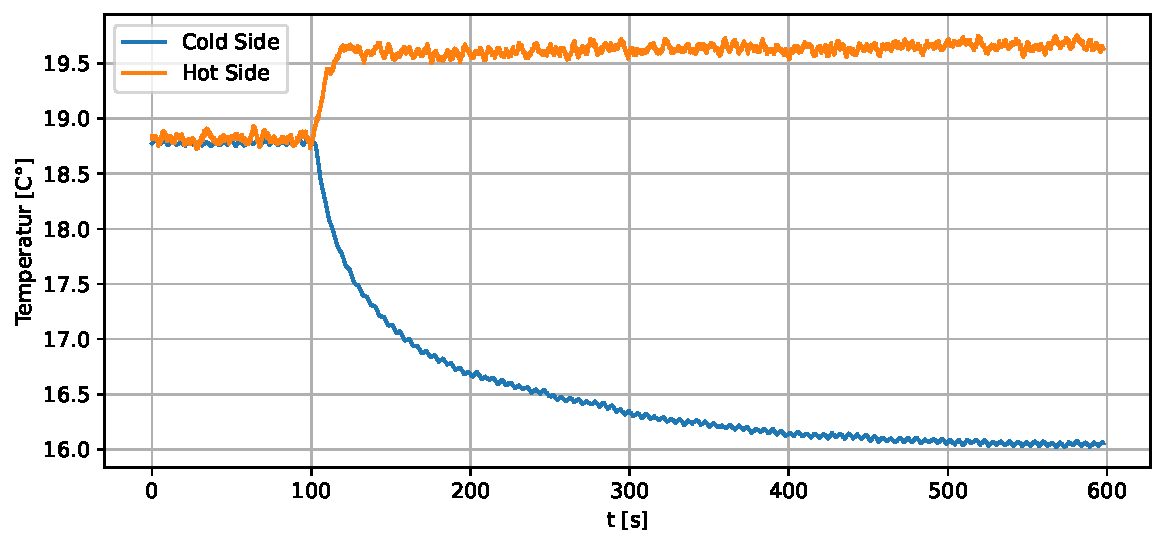
\includegraphics[width=\linewidth]{kapitel4/images/stepFührungsgröße}}
\caption{stepFührungsgröße}
\label{Grundlagen:stepFührungsgröße}
\end{figure}

\begin{figure}[H]
\makebox[\textwidth]{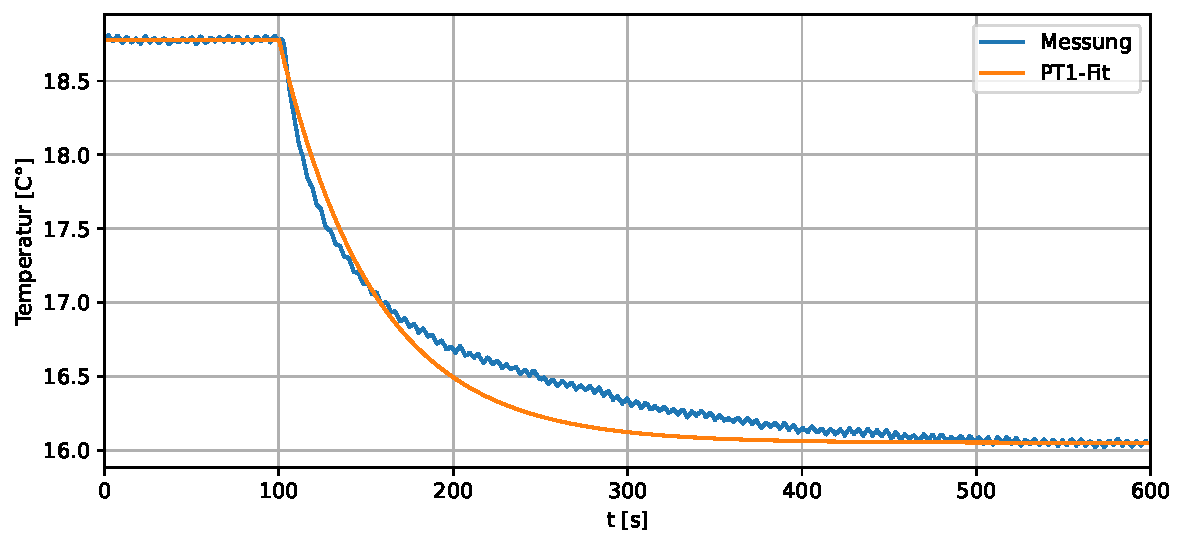
\includegraphics[width=\linewidth]{kapitel4/images/stepFührungsgrößePT1Fit}}
\caption{stepFührungsgrößePT1Fit}
\label{Grundlagen:stepFührungsgrößePT1Fit}
\end{figure}


\section{PI-Regler}
Im folgendem soll ein geeigneter Regler gefunden werden.
\begin{figure}[H]
\makebox[\textwidth]{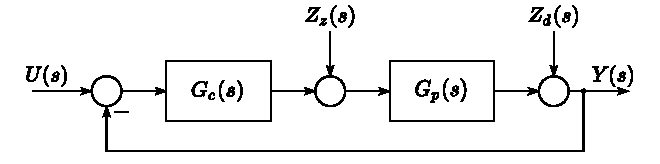
\includegraphics[width=\linewidth]{kapitel4/images/Regelkreis}}
\caption{Regelkreis}
\label{Grundlagen:Regelkreis}
\end{figure}
Für die zu regelnde Strecke wird ein PT1 Glied mit der folgenden Form angenommen.
\begin{equation}
	G_P(s) = K_P\frac{T_N}{s+T_N}
\end{equation}
Die Strecke wird über die stationäre Verstärkung $K_P$ und die Zeitkonstante $T_N$ parametriert, die bereits aus der Messung des Führungseinheitssprunges bekannt sind. Der geschlossene Regelkreis soll einen bleibenden Regelfehler vermeiden und als Führungssprung mit einem frei wählbaren PT1 verhalten antworten. Für die Reglerstruktur werden dementsprechend eine Nussstelle, zum kompensieren der Eigendynamik, und ein Integrator, für die bleibende Regelabweichung, benötigt. Die geforderte Struktur ist durch einen PI-Regler realisierbar.
\begin{equation}
	G_c(s) = K_C \frac{s + \beta}{s}
\end{equation}
Ziel ist es die Eigendynamik des Systems zu kompensieren und ein frei bestimmbares PT1 Verhalten vorzugeben. Für die Kompensation des Pols der Strecke wird die Nullstelle des Reglers verwendet. Es folgt also $\beta = T_N$. Damit ergibt sich der offene Regelkreis zu
\begin{equation}
	L(s) = \frac{K_C K_P T_N}{s}
\end{equation}
Da der offene Regelkreis ein Integrator aufweist gilt
\begin{equation}
	e_\infty = 0
\end{equation}
Der geschlossene Regelkreis ergibt sich zu 
\begin{equation}
	T(s) = \frac{L(s)}{1+L(s)} = \frac{K_C K_P T_N}{s + K_C K_P T_N}
\end{equation}
Mit $K_C$ als frei wählbarer Parameter kann eine beliebiges PT1 verhalten vorgegeben werden. Da für gewöhnlich ein rein statischer Sollwert vorgegeben wird, sind die Störübertragungsfunktionen von größerer Bedeutung. Da die erwartete Störgröße an dem Streckenausgang wirkt soll im folgendem die Störübertragung betrachtet werden.
\begin{equation}
\frac{Y}{Z_d} = \frac{s}{s+K_CK_PT_N}
\end{equation}
Es ist ersichtlich, dass für $t\rightarrow\infty$ die Störgrößeneinwirkung vollständig kompensiert wird. Die Dynamik der Störübertragung kann durch Vorgabe von $K_C$ Parametriert werden. Da es sich um einen 1-DOF (degree of freedom) Regler handelt, kann kein individuelle Übertragungsfunktion für Führungs- und Störverhalten gefunden werden. Die Verwendung eines 2-DOF Regler ist nicht Notwendig da nur das Störverhalten von Interesse ist. Die folgende Abbildung zeigt die wirkende Störgröße am Streckenausgang mit einer Übertragungsfunktion $G_z(s)$.
\begin{figure}[H]
\makebox[\textwidth]{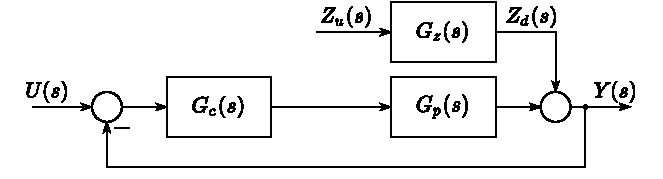
\includegraphics[width=\linewidth]{kapitel4/images/RegelkreisStörgröße}}
\caption{Regelkreis mit wirkender Störgröße}
\label{Grundlagen:RegelkreisStörgröße}
\end{figure}
Falls die Störgröße $Z_u(s)$ und die Übertragungsfunktion $G_z(s)$ bekannt sind kann die Störgröße vollständig kompensiert werden. 
\begin{figure}[H]
\makebox[\textwidth]{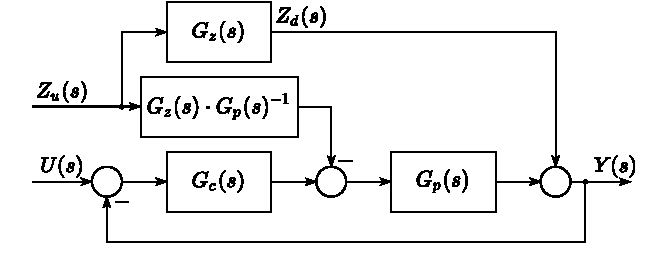
\includegraphics[width=\linewidth]{kapitel4/images/RegelkreisStörgrößeKompensiert}}
\caption{Regelkreis mit kompensierter Störgröße}
\label{Grundlagen:RegelkreisStörgrößeKompensiert}
\end{figure}